\documentclass{llncs}
\usepackage{amsmath,amssymb}
\usepackage{url}
\usepackage{overpic}
\usepackage{enumerate}
\usepackage{graphicx}        % standard LaTeX graphics tool
\usepackage{tikz}        % standard LaTeX graphics tool
\usepackage{subfigure}                                 % authors: subfigures
\usepackage[ruled,vlined,linesnumbered]{algorithm2e}   % authors: last version of algorithm display
\usepackage{todonotes}
\usepackage[ruled,vlined,linesnumbered]{algorithm2e}


%\title{A Subquadratic and Separable Algorithm for Chamfer Norm
  %Distance Transformation \thanks{This work has been mainly funded
  %  by  ANR-11-BS02-009 and  ANR-11-IDEX-0007-02 PALSE/2013/21 research grants.}}



\title{Generic Separable Algorithms for Distance Transformation: A
  Subquadratic Approach for Path Based Norms\thanks{This work has been
    mainly funded by ANR-11-BS02-009 and ANR-11-IDEX-0007-02
    PALSE/2013/21 research grants.}}

\author{David Coeurjolly\inst{1}}

 \institute{ CNRS,  LIRIS, UMR5205, F-69621, France\\
   \email{david.coeurjolly@liris.cnrs.fr}
}
\graphicspath{{./Figs/}}
%fonts bonanza
\usepackage{amsmath,amssymb,amsfonts}
\usepackage{pifont}% http://ctan.org/pkg/pifont
\newcommand{\CheckMark}{\ding{51}}%
\newcommand{\CrossMark}{\ding{55}}%
% Zapf font
\usepackage[mathscr]{euscript}
\DeclareFontFamily{OT1}{pzc}{}
\DeclareFontShape{OT1}{pzc}{m}{it}%
              {<-> s * [1.2] pzcmi7t}{}
\DeclareMathAlphabet{\mathpzc}{OT1}{pzc}{m}{it}
% rescaling cal to be a touch smaller
\DeclareFontFamily{OMS}{fcmsy}{\skewchar\font48 }
\DeclareFontShape{OMS}{fcmsy}{m}{n}{%
         <-5.5> [.96] cmsy5     <5.5-6.5> [.96] cmsy6
      <6.5-7.5> [.96] cmsy7     <7.5-8.5> [.96] cmsy8
      <8.5-9.5> [.96] cmsy9     <9.5->  [.96] cmsy10
      }{}
\DeclareFontShape{OMS}{fcmsy}{b}{n}{%
       <-6> [.96] cmbsy5
      <6-8> [.96] cmbsy7
      <8->  [.96] cmbsy10
      }{}
\DeclareMathAlphabet{\mathcal}{OMS}{fcmsy}{m}{n}
\usepackage{bbm}

\usepackage{mathtools}% http://ctan.org/pkg/mathtools
\usepackage{calc}% http://ctan.org/pkg/calc

\newcommand*{\mytilde}[2][0pt]{%
  \setbox0=\hbox{$#2$}%
  \tilde{\mathrlap{\phantom{\rule{\wd0}{\ht0+{#1}}}}\smash{#2}}%
}
\newcommand*{\mywidetilde}[2][0pt]{%
  \setbox0=\hbox{$#2$}%
  \widetilde{\mathrlap{\phantom{\rule{\wd0}{\ht0+{#1}}}}\smash{#2}}%
}

%%Space, Lattices
\newcommand{\Z}{{\mathbb{Z}}}
\newcommand{\R}{{\mathbb{R}}}

%%Formulas
\newcommand{\EqDef}{\!\ensuremath{\mathrel{\mathop:}=}\!}
%\newcommand{\EqDef}{\smash{\ensuremath{\stackrel{\text{def}}{=}}}}

%% Misc.
\newcommand{\txtblue}[1]{\textcolor{blue}{ #1}}
\newcommand{\txtgreen}[1]{\textcolor{green}{ #1}}
\newcommand{\txtred}[1]{\textcolor{red}{ #1}}

\begin{document}
\maketitle


\begin{abstract}
In many applications, separable algorithms have demonstrated their
efficiency to perform high performance volumetric computations, such
as distance transformation or medial axis extraction. In the
literature, several authors have discussed about the conditions on the
metric to be considered in a separable approach.  In this article, we
present generic separable algorithms to efficiently compute Voronoi
maps and distance transformations for a large class of
metrics. Focusing to path based norms (chamfer masks, neighborhood
sequences, ...), we detail a subquadratic algorithm to compute such
volumetric transformations. More precisely, we describe a
$O(N\log^2(m))$ algorithm in dimension 2 for shapes with $N$ grid
points and for example a chamfer mask of size $m$.

\keywords{Digital Geometry, Distance Transformation, Chamfer Norms}
\end{abstract}

\section{Introduction}
\label{sec:introduction}

Since early works on digital geometry, distance transformation plays
an important role in many applications
\cite{Rosenfeld1966,Rosenfeld1968}. Given a finite input shape
$X\subset \Z^n$, the distance transformation labels each point in $X$
with the distance to the closest point in $\Z^n \setminus X$. Since
such characterization is parametrized by a distance function, many
works have been done to address this distance transformation problem
with a trade-off between algorithmic performances and the
\emph{accuracy} of the digital distance function with respect to the
Euclidean one.  Hence, authors have considered distances based on
chamfer masks
\cite{Rosenfeld1968,borgefors,Thiel_IWCIA7,fouard:ivc:2005} or
sequences of chamfer masks
\cite{ROSEN_66,mukherjee,Nagy05,Strand2008,DBLP:conf/dgci/NormandSE13};
the vector displacement based Euclidean distance
\cite{danielson,ragnemalm,MULL_92,Cuisenaire1999_268}; the Voronoi
diagram based Euclidean distance
\cite{BreuEtAl95,maurer_pami} or the square of the
Euclidean distance \cite{SaitTori:94,Hirata,roerdnik}.

\paragraph{Contributions} In this article,



\begin{table}
  \caption{Complexity summary.}
  \label{tab:final}
  \begin{center}
    \begin{tabular}{|c|c|c|c|c|}
      \hline
      Metric &\textsc{Closest}& \textsc{HiddenBy} & Sep. Voronoi Map & Reference\\
      \hline
      $L_2$ & $O(1)$ &  $O(1)$ & $\Theta(n\cdot N^n)$ & \cite{Hirata1996}\\
      $L_\infty$ & $O(1)$ & $O(1)$ &  $\Theta(n\cdot N^n)$ & \cite{roerdnik}\\
      $L_1$ & $O(1)$ &   $O(1)$ &$\Theta(n\cdot N^n)$& \cite{roerdnik}\\
      $L_p$  (exact pred.) & $O(\log{p})$ &
      $O(\log{p}\cdot\log{N})$ & $O(n\cdot
      N^n\cdot\log{p}\cdot\log{N})$& here and  \cite{dgtal}\\
      $L_p$  (inexact pred.) & $O(1)$ &
      $O(\log{N})$ & $O(n\cdot
      N^n\cdot\log{N})$& here and  \cite{dgtal}\\
      2D Chamfer norm &  $O(\log{m})$ &$O(\log^2{m})$
      &$O(\log^2{m}\cdot N^2)$& Theorem \ref{them}\\
      3D Chamfer norm &  $O(\log{m})$ &$O(\log^2{m})$
      &$O(\log^2{m}\cdot N^3)$& Theorem \ref{them2}\\
      nD Chamfer norm &  $O(n\cdot\log{f})$ &$O(n\cdot log^2{f}\cdot\log{N})$
      & $O(n^2\cdot N^n\cdot \log{f}\cdot\log{N})$& Corollary \ref{coro2}\\
      2D Neig. sequence norm  & $O(\log{m})$&
      $O(\log^2{m})$& $O(\log^2{m}\cdot N^2)$& Theorem \ref{them} and  \cite{DBLP:conf/dgci/NormandSE13}\\
      \hline
    \end{tabular}
  \end{center}
\end{table}

\section{Preliminaries}
\label{sec:preliminaries}

Let us first define some elementary concepts and objects.
\begin{definition}[Metrics and Metric Space]
  \label{def:distance}
  A metric is a map $d$ from $E$ to a sub-group $F$ of $\R$ such that
  $\forall a,b,c\in E$,
  \begin{align}
    (\text{non-negative})\quad & d(a,b)\geq 0\\
    (\text{identity of indiscernibles}) \quad&  d(a,b)= 0
    \Leftrightarrow a=b\\
    (\text{symmetry})\quad &  d(a,b)=d(b,a)\\
    (\text{triangular inequality})\quad &   d(a,c) \leq d(a,b) + d(b,c)
  \end{align}
$(E, F, d)$ is called a metric space.
\end{definition}
If property $(4)$ is omitted, we are defining a distance function
instead of a metric. Note that in the following, we will only consider
metric spaces with properties $(1-4)$. Furthermore, we may have to
consider  metrics induced by a vector space norm:
\begin{definition}[Norm and metric induced by a norm]
  \label{def:distance}
  Given a vector space EV, a norm is a map $g$ from  $EV$ to a sub-group
  $F$ of $\R$ such that $\forall \vec{x},\vec{y}\in EV$,
  \begin{align}
    (\text{non-negative})\quad & g(\vec{x})\geq 0\\
    (\text{identity of indiscernibles}) \quad&  g(\vec{x})= 0
    \Leftrightarrow \vec{x}=\vec{0}\\
    (\text{triangular inequality})\quad &   g(\vec{x}+\vec{y}) \leq
    g(\vec{x}) + g(\vec{y})\\
    (\text{homogeneity})\quad &  \forall \lambda\in\R, \quad
    g(\lambda\cdot\vec{x}) = |\lambda|\cdot g(\lambda\cdot\vec{x})
  \end{align}
$d(a,b) \EqDef g(b-a)$ is the metric induced by the
  norm $g$.
\end{definition}
Note that the above definition can be extended from vector spaces to
\emph{modules} on a commutative ring ($\Z^n$ being a module on $\Z$
but not a vector space) \cite{Thiel_hdr}.

From the literature, path-based approaches (Chamfer masks, (weighted)
neighborhood sequences...)  aim at defining metrics induced by norms
in metric spaces $(\Z^n, \Z , d)$.  Note that (weighed, with $w_i\geq 0$) $L_p$ norms inducing
metrics
\begin{equation}
    d_{\ell_p} (a,b) = \left ( \sum_{i=0}^n w_i|a_i-b_i |^p \right )^{\frac{1}{p}}\,
  \end{equation}
characterize metric spaces $(\Z^n, \R , d_{\ell_p})$. However,
rounding the metric $(\Z^n,\Z, \lceil d_{\ell_p}\rceil)$ implies a
metric space \cite{klette_book}.

\begin{definition}[Distance Transformation and Voronoi Map]
  The distance transform $DT_X$ associated with a digital metric space
  $(\Z^n,\Z,d)$ is a map  $X\rightarrow\Z$ such that
  \begin{equation}
    DT_X(a) = \min_{b\in \Z^n\setminus X} \{d(a,b)\}
  \end{equation}
The Voronoi map is the map $X\rightarrow\Z^n$:
  \begin{equation}
    \Pi_X(a) = \argmin_{b\in \Z^n\setminus X} \{d(a,b)\}
  \end{equation}
\end{definition}
Voronoi map $\Pi_X$ corresponds to the intersection between the
continuous Voronoi diagram for the metric $d$ of points
$\Z^n\setminus$ and the lattice $\Z^n$. If a digital point $a$ belongs
to a Voronoi diagram $d-$facet ($1\leq d< n$), $a$ is equidistant to 2
or more points in $\Z^n\setminus X$ but only one is considered in
$\Pi_X(a)$ (please refer to\cite{Couprie2007} for complete digital
Voronoi map construction).

\begin{definition}[Chamfer Mask]
  A weighted vector is a pair $(\vec{v},w)$ with $\vec{v}\in\Z^n$ and
  $w\in\N^*$. A chamfer mask $\M$ is a central-symmetric set of weighted
  vectors with non-empty vectors and containing at least a basis of
  $\Z^n$.
\end{definition}

In the literature
\cite{borgefors,Thiel_hdr,Strand2008,normandHDR,fouard:ivc:2005} many
authors have proposed algorithmic and/or analytic approaches to
construct Chamfer masks approximating the Euclidean metric and being
induced by norm. In the following, we focus on such \emph{chamfer
  norms}.  To evaluate distances between two digital points for a
given chamfer metric, direct formulations have been proposed with
simple geometrical interpretation:
\begin{definition}[Rational ball, minimal H-representation \cite{Thiel_hdr,DBLP:journals/pr/NormandE09}]
  Given a Chamfer mask $\M$ inducing a norm, the rational ball
  associated with $\M$ is the polytope
  \begin{equation}
\label{eq:4}
    \B = conv\left\{ \frac{\vec{v}_i}{w_i};\; (\vec{v}_i,w_i)\in\M \right \}\,.
  \end{equation}
Rational ball $\B$ can also be described in a H-representation of
polytope with minimal parameter \cite{DBLP:conf/dgci/NormandSE13}
\begin{equation}
  P = \{ x\in\Z^n; Ax \leq y\;\}\quad \text{ such that }  \forall
  i\in[1\ldots l], \exists x\in P\quad A_ix=y_i\,.\footnote{$A_i$
    being the $i^{th}$ row of $A$.}
\end{equation}
$l$ being the number of row in $A$ and the number of facets in $\B$,   and is thus related to $|\M|$.
\end{definition}

An important result for distance computation can be formalized as follows:
\begin{proposition}[Direct Distance Computation \cite{DBLP:journals/pr/NormandE09}]
  Given a chamfer mask $\M$ inducing a norm and $(A,y)$ its minimal
  parameter H-representation, then for any $a\in\Z^n$, the chamfer
  distance of $a$ from the origin is
  \begin{equation}
    \label{eq:1}
    d_\M(O,a) =  \max_{1\leq i \leq l} \{ A_i a^T\}\,.
  \end{equation}
\end{proposition}


Among path-based digital metric, we can also introduce (weighted)
neighborhood sequences
\cite{ROSEN_66,mukherjee,Nagy05,Strand2008,DBLP:conf/dgci/NormandSE13}
whose objective is to have better approximation of the Euclidean
metric from sequences of elementary chamfer masks.  A key result have
been demonstrated in \cite{DBLP:journals/pr/NormandE09} stating
that for such distance functions, a minimal parameter polytope
representation exists and that distances can be from similar
expression to (\ref{eq:1}):
\begin{equation}
  d(O,a)  =\max_{1\leq i \leq l} \{ f_i(A_i a^T)\}\,,
\end{equation}
($f_i$ being and integer sequence characterizing the neighborhood
sequence metric).


 In the following and for the sake of simplicity, we describe our
 algorithms focusing to chamfer norms but similar results can be
 obtained for more generic path-based metric such neighborhood
 sequences.

\section{Separable Distance Transformation}
\label{sec:separ-dist-transf}



\subsection{Voronoi Map from Separable Approach and Metric Conditions}
\label{sec:voronoi-map-from}

In \cite{Hirata1996,SaitTori:94,Breu1995,Meijster2000,Maurer2003},
several authors have described optimal in time and separable
techniques to compute error-free Voronoi maps or distance
transformations for $L_2$ and $L_p$ metrics. Separability means that
computations are performed dimension by dimension, allowing fast
computations and multithread implementations (see
\cite{dcoeurjo_ChapDT} for an overview).  In the following, we
consider Voronoi map approach as defined in \cite{Breu1995} (see
Fig.~\ref{fig:2Dbreu}): Let us first define hyper-rectangular domain
$I_X: [0..N_1]\times\ldots[0..N_n] \rightarrow \{0,1\}$ such that
$X\subset I_X$ and $I_X(a)= 1$ for $a\in [0..N_1]\times\ldots[0..N_n]$
iff $a\in X$ ($I_X(a)=0$ otherwise). As illustrated in
Fig.~\ref{fig:2Dbreu} in dimension 2, we first process each row of the
input image to create independent 1D Voronoi maps along the first
dimension for the metric. Then, for each further dimension, the
partial Voronoi map $\Pi_X$ is updated using one dimensional
independent processes on image spans along the $i^{th}$
dimension.

\begin{algorithm}[H]\small
  \KwData{Input binary map $I_X$ if $i=1$ or  partial Voronoi map $\Pi_X$ obtained for
    dimension $1<j<i$, and a 1D segment $S$ with points
    $\{s_1,\ldots,s_{N_i}\}$ sorted by their $i^{th}$ coordinate.}
  \KwResult{Updated partial Voronoi map $\Pi_X$ along $S$.}
\If{ i = 1}
{ $k=0$\;
\ForEach{point $s_i$ in $S$}{
    \If{$I_X(s_i) = 1$}
     {
       $L_S[k] = s_i$\;
       $k++$\;
     }
}
}
\Else{
 ${L}_S[0]=\Pi_X(s_1)$\;
  ${L}_S[1]=\Pi_X(s_2)$\;
  $k=2$ , $l=3$\;
  \While{$l\leq N_i$}{
    $w = \Pi_X(s_l)$\;
    \While{$k\geq 2$ and \textsc{HiddenBy}(${L}_S[k-1],{L}_S[k],w, S$)}
          {
         $ k--$\;
        }
        $k++$ , $l++$\;
        ${L}_S[k]=w$\;
  }
}
  \ForEach{point  $s$ in $S$ by increasing $i^{th}$ component}
  {
    \While{($k < |L_S|$) and not(\textsc{Closest}($s$, $L_S[k]$, $L_S[k+1]$))}
          {
            $k++$\;
          }
    $\Pi_X[s] = L_S[k]$\;
  }

  \caption{Voronoi map pruning along 1D segment $S$ along the $i^{th}$
    dimension.\label{alg:voro}}
\end{algorithm}

\begin{figure}
  \begin{center}
     \begin{overpic}[draft=false,width=10cm]{figs/edt_dcoeurjo}
       \put(30,5){$Candidates_S$}
       \put(57,0){$S$}
     \end{overpic}
  \end{center}
  \caption{Voronoi Map construction in dimension 2.\label{fig:2Dbreu}}
\end{figure}


Algorithm \ref{alg:voro} describe the 1D processes to perform on each
row, columns and higher dimension spans. In this process, metric
information are embedded in the following two predicates:
\begin{itemize}
  \item \textsc{Closest}$(a, b, c)$: given three points $a,b,c\in\Z^n$
    this predicate returns true if $d(a,b) < d(a,c)$ ;
  \item \textsc{HiddenBy}$(a, b, c, S)$: given three points
    $a,b,c\in\Z^n$ such that $a_i<b_i<c_i$ and a 1D image span $S^i$, this predicates returns
    true if there is no  $s\in S$ such that
    \begin{equation}
      d(b,s) < d(a,s)\text{ and }  d(b,s) < d(c,s)\,.
    \end{equation}
\end{itemize}
In other words, \textsc{HiddenBy} returns true if and only if the
Voronoi cell of sites $a$ and $c$ \emph{hide} the Voronoi cell of $b$
along $S$ (\emph{e.g.} $A$ and $E$ \emph{hide} $C$ and $B$ on $S$ in
Fig.~\ref{fig:2Dbreu}).  For $L_1$, $L_2$ and $L_\infty$ metrics,
\textsc{Closest} and \textsc{HiddenBy} predicates can be computed in
$O(1)$ \cite{Breu1995,Hirata1996,Meijster2000}. Hence, Algorithm
\ref{alg:voro} is in $O(N_i)$ for dimension $i$, leading to an overall
computational time for the Voronoi map and distance transformation
problem in $O(n\cdot N^n)$ (if we assume that $\forall i\in[1\ldots
  n], N_i=N$).

In \cite{Hirata1996} or \cite{maurer_pami}, authors discussed about
conditions on the metric $d$ to ensure that Algorithm \ref{alg:voro}
is correct. The key property can be informally describe as follows:
given two points $a,b\in\Z^n$ such that $a_i<b_i$ and a straight line
$l$ along the $i^{th}$ direction and if we denote by $v_l(a)$
(resp. $v_l(b)$) the intersection between the Voronoi cell of $a$
(resp. $b$) and l, then $v_l(a)$ and $v_l(b)$ are simply connected
Euclidean segments and $v_l(a)$ appears \emph{before} $v_l(b)$ on $l$
(so called \emph{monotonicity property} in \cite{Maurer2003} and is
related to \emph{quadrangle inequality} in \cite{Hirata1996}).  To sum
up these contributions, we use the following proposition:
\begin{proposition}[Metric conditions \cite{Hirata1996}]
\label{prop:voronoi-map-from-1}
  Let $d$ be a metric induced by a norm whose unit ball is symmetric
  with respect to grid axis. If distance comparison predicate
  $d(a,b)<d(c,d)$ is exact (for $a,b,c,d\in\Z^n$), Algorithm 1 is
  correct and returns a Voronoi map $\Pi_X$.
\end{proposition}

For example, Algorithm \ref{alg:voro} provides exact Voronoi map
computation for $L_p$ norms. In such case, distance comparison
predicate can be implemented error-free form integer number comparison
considering the $p$ power of the distance function $\left
(d_{L_p}\right)^p$.  Proposition \ref{prop:voronoi-map-from-1} also
implies that Chamfer norms, neighborhood sequences based norms can
also be considered in separable Algorithm \ref{alg:voro}. We just need
algorithmic tools to implement efficiently both \textsc{Closest} and
\textsc{HiddenBy} predicates.

\subsection{A First Generic Adapter}
\label{sec:first-gener-adapt}

Let suppose that $(\Z^n,F,d)$ is a metric space induced by a norm. We
can first detail the overall computational cost of Algorithm
\ref{alg:voro}:

\begin{lemma}
\label{lem:generic}
   Let $(\Z^n, F, d)$ be a metric space induced by a norm. If $C$
  denotes the computational cost of \textsc{Closest} predicate and $H$
  is the computational cost of the \textsc{HiddenBy} predicate, then
  Algorithm \ref{alg:voro} is in
  \begin{equation}
    O(n\cdot N^n\cdot (C+H))\;.
  \end{equation}
\end{lemma}


A first improvement is given by Algorithms~\ref{alg:genclosest},
\ref{alg:genedge} and \ref{alg:genhidden}: we only require the metric
to be known and \textsc{HiddenBy} predicate is obtained by a binary
search on the 1D image span $S$ to localize the abscissa of Voronoi
edges of sites $(a,b)$ and $(b,c)$ (see Fig.XXXXXX). Please note that
from \cite{Breu1995,roerdnik}, $C=H=O(1)$ for $L_1,L_2$ and $L_\infty$
norms.



\begin{algorithm}[H]\small
  \Return $d(a,b) < d(a,c)$\;
  \caption{Generic \textsc{Closest}($a,b,c\in\Z^n$).\label{alg:genclosest}}
\end{algorithm}


\begin{algorithm}[H]\small
  \If{$(j-i=1)$}
     {
       \Return  i
     }
     $mid  = i + (j-i)/2$\;
     \eIf{\textsc{Closest}$(s_{mid},a,b)$}
       {
         \tcp{$s_{mid}$ closer to $a$}
         \Return \textsc{VoronoiEdge}($a,b,s_{mid},s_j$)
}
 {
         \tcp{$s_{mid}$ closer to $b$}
         \Return \textsc{VoronoiEdge}($a,b,s_{i},s_{mid}$)
}

  \caption{Generic \textsc{VoronoiEdge}($a,b,s_i,s_j\in\Z^n$).\label{alg:genedge}}
\end{algorithm}

\begin{algorithm}[H]\small
  $v_{ab}$ = \textsc{VoronoiEdge}$(a,b,s_1, s_{N_i})$\;
  $v_{bc}$ = \textsc{VoronoiEdge}$(b,c,s_1, s_{N_i})$\;
  \Return $(v_{ab}> v_{bc})$\;
  \caption{Generic \textsc{HiddenBy}($a,b,c\in\Z^n; S$ in the $i^{th}$
    direction).\label{alg:genhidden}}
\end{algorithm}

Hence, we obtain a first generic metric adapter to transform it into
separable predicates:

\begin{lemma}
\label{lem:generic}
   Let $(\Z^n, F, d)$ be a metric space induced by a norm. If $C$
   denotes the computational cost of \textsc{Closest} predicate
   Algorithm \ref{alg:voro},  with predicates from Algorithms
   \ref{alg:genclosest} and \ref{alg:genhidden}, is in
  \begin{equation}
    O(n\cdot N^n\cdot C\cdot \log{N}))\;.
  \end{equation}
\end{lemma}

If we consider a chamfer norm with $l$ facet unit ball, Eq.~(\ref{eq:1})
suggests that $C=O(l)$. Hence, we have the following corollary
\begin{corollary}
  Let $\M$ be a chamfer norm whose rational ball has $l$ facets,
  separable exact Voronoi map $\Pi_X$ can be obtained in
 \begin{equation}
    O(n\cdot N^n\cdot l \cdot \log{N}))\;.
  \end{equation}
\end{corollary}

Please remember that naive implementation of chamfer mask distance
transformation using raster scan approach would lead to a $O(l\cdot
N^d)$ computational cost. In the following sections, we use the convex
structure of $\B$ to design a first subquadratic algorithm for chamfer
norms.

\subsection{Subquadratic Algorithm in Dimension 2}
\label{sec:subq-algor-dimens}

Let us consider a 2D chamfer norm $\M$ with $m$ weighted vectors (note
that $l\EqDef|\B| = m$ in 2D). We suppose that vectors
$\{v_k\}_{k=1\ldots m}$ are sorted counterclockwise. We define a wedge
as a pair $(\vec{v_k},\vec{v_{k+1}})$ of vectors. To each wedge is
associated a row $A_k$ in the minimal H-representation of $A$ ($A_k$
can also be seen as a non-unit normal vectors to $\B$
facets\cite{DBLP:journals/pr/NormandE09})

Using these notations, \cite{Thiel_hdr,Strand2008} demonstrate that
the distance evaluation of point $a$ can be obtained in two steps:
First, we compute the wedge $(\vec{v_k},\vec{v_{k+1}})$, $a$ belongs
to. Then,
\begin{equation}
\label{eq:2}
  d_\M(O,a) = A_k\cdot a^T
\end{equation}

\begin{lemma}
\label{lem:log}
  Given a chamfer norm $\M$ in dimension 2 with $m$ vectors, the distance computation
  and thus the \textsc{Closest} predicate are in $O(\log{m})$.
\end{lemma}
\begin{proof}
  Since vectors are sorted counter-clockwise,
  $(\vec{v_k},\vec{v_{k+1}})$ wedge can be obtained by a dichotomic
  search with $O(\log{m})$ steps. At each step, we compute the local
  orientation of point $a$ w.r.t. a direction which is in $O(1)$. Once
  the wedge has been obtained, Eq.~(\ref{eq:2}) returns the distance
  value in $O(1)$.$\Box$
\end{proof}

Please note that in practical implementations, we can use symmetries
in $\M$ vectors to only work on restrictions of chamfer mask
directions.

To optimize the \textsc{HiddenBy} predicate, we focus on the
\textsc{VoronoiEdge} function. Given two points $a$ and $b$
($a_i<b_i$) and a 1D image span $S$ along the $i^{th}$ dimension, we
can to find the lowest abscissa $e_i$ of the point $e$ on $S$ such
that $d(a,e) < d(b,e)$ and $d(a,e')\geq d(b, e')$ for any $e'$ with
$e'_i>e_i$.

Let us first suppose that we don't have $e$ but we know the wedges
$(v_{k},v_{k+1})$ (resp. $(v_j,v_{j+1})$) such that the vector
$(e-a)^T$ (resp. $(e-b)^T$) should belong to (see Fig.XXXXX). In this
situation, we know that $e$ is the solution of
\begin{equation}
\label{eq:3}
  A_k\cdot  (e-a)^T = A_j\cdot (e -b)^T\;.
\end{equation}
(since $e\in S$, we have one linear equation for one unknown
$e_i$). As a consequence, if we know the wedges the Voronoi edge
belongs to, we have the abscissa in $O(1)$ (see Algorithm \ref{alg:chamedge}).
\begin{algorithm}[h]\small
  $(v_k,v_{k+1})$ = \textsc{VoronoiEdgeWedge}$(a,b,\vec{v}_1,\vec{v}_m, S)$\;
  $(v_j,v_{j+1})$ = \textsc{VoronoiEdgeWedge}$(b,a,\vec{v}_1,\vec{v}_m, S)$\;

  Compute the abscissa $e_i$ of the point $e$ such that $A_k\cdot
  (e-a)^T = A_j\cdot (e -b)^T$\;

  \Return $e_i$\;
  \caption{2D chamfer norm \textsc{VoronoiEdge}($a,b,s_i,s_j\in\Z^2$).\label{alg:chamedge}}
\end{algorithm}
To obtain both wedges, we use a dichotomic search similar to
Algorithm~\ref{alg:genedge}: Algorithm~\ref{alg:chamedgew} returns the
wedge associated to $a$ containing the Voronoi edge with respect to
$b$. Applying this algorithm to obtain the $b$ wedge with respect to
$a$ gives exactly  Algorithm \ref{alg:chamedge}.

The dichotomic search shrinks the set of vectors
$\{\vec{v}_i,\ldots,\vec{v}_j\}$ to end up is a wedge $(v_k,v_{k+1})$
such that the intersection point between the straight line $(a +
\vec{v}_k)$ and $S$ is in the Voronoi cell of $a$ and such that the
intersection between $(a + \vec{v}_k)$ and $S$ is in the Voronoi cell
of $b$. Algorithm~\ref{alg:chamedgew} thus first compute the
intersection points associated with a wedge $(\vec{v}_{i+(j-i)/2},
\vec{v}_{i+(j-i)/2+1})$ (lines $5-6$); Evaluates the distances at
these points (lines $7-8$) and then decides which set
$\{\vec{v}_i,\ldots,\vec{v}_{i+(j-i)/2}\}$ or
$\{\vec{v}_{i+(j-i)/2},\ldots,\vec{v}_j\}$ has to be considered for
the recursive call (lines $14-25$).

\begin{algorithm}
\small
  \eIf{ $(j-i =1)$}{
    \Return $(\vec{v}_k,\vec{v}_{k+1})$\;}
{
   $mid  = i + (j-i)/2$\;
   Let $p_{mid}$  be the intersection point between $(a +
   \vec{v}_{mid})$ and $S$\;
  Let $p_{mid+1}$  be the intersection point between $(a +
   \vec{v}_{mid+1})$ and $S$\;


   \tcp*[f]{$O(1)$ evaluation of distances w.r.t. $a$}
   $d^a_{p_{mid}} = A_{mid}\cdot (p_{mid}-e)^T$\;
   $d^a_{p_{mid+1}} = A_{mid+1}\cdot (p_{mid+1}-e)^T$\;


   \tcp*[f]{$O(\log{m})$ evaluation of distances w.r.t. $b$}
   $d^b_{p_{mid}} = d_\M(b, p_{mid})$\;
   $d^b_{p_{mid+1}} = d_\M(b,p_{mid+1})$\;

   Let $b_{mid}$ be true if $d^a_{p_{mid}} < d^b_{p_{mid}}$; false otherwise\;
   Let $b_{mid+1}$ be true if $d^a_{p_{mid+1}} < d^b_{p_{mid+1}}$; false otherwise\;


   \If{ $b_{mid}\neq b_{mid+1}$ \tcp*[r]{we have the Voronoi edge
       wedge}} { \Return $(\vec{v}_{mid},\vec{v}_{mid+1})$\; }

    \If{ $b_{mid}=b_{mid+1}=true$ \tcp*[r]{Both points are in $a$'s cell}}
{
    \eIf{$a_i < b_i$}
{
  \Return \textsc{VoronoiEdgeWedge}$(a,b,\vec{v}_{mid}, \vec{v}_{j}, S)$\;
}
{
  \Return \textsc{VoronoiEdgeWedge}$(a,b,\vec{v}_{i}, \vec{v}_{mid}, S)$\;
}

}
    \If{ $b_{mid}= b_{mid+1}=false$\tcp*[r]{Both points are in $b$'s cell}}
{
    \eIf{$a_i < b_i$}
{
  \Return \textsc{VoronoiEdgeWedge}$(a,b,\vec{v}_{i}, \vec{v}_{mid}, S)$\;
}
{
  \Return \textsc{VoronoiEdgeWedge}$(a,b,\vec{v}_{mid}, \vec{v}_{j}, S)$\;
}

}

}
  \caption{\textsc{VoronoiEdgeWedge}($a,b\in\Z^2; \vec{v}_i,\vec{v}_j$
    in $\M$; $S$ along the $i^{th}$ direction).\label{alg:chamedgew}}
\end{algorithm}


\begin{theorem}
\label{them}
  Let $\M$ be a 2D chamfer norm with $m$ weighted vectors, then we
  have
  \begin{enumerate}[(i)]
  \item Algorithm     \ref{alg:chamedge} is   $O(\log^2{m})$\;;
  \item Algorithm \ref{alg:voro} (with predicates from Algorithms
    \ref{alg:chamedge} and Lemma \ref{lem:log}), computes a Voronoi
    map $\Pi_X$ and thus the distance transformation of $X$ for metric
    $d_{M}$ in
  \begin{equation}
    O( \log^2{m}\cdot N^2)\;.
  \end{equation}
  \end{enumerate}
\end{theorem}
\begin{proof}
Let us first consider statement $(i)$. As described above, Algorithm
\ref{alg:chamedgew} performs $\log{m}$ recursive calls and each step
is in $O(\log{m})$. Indeed, $p_{mid}$ and $p_{mid+1}$ are given by the
intersections between two rational slope straight lines plus a
rounding operation on fractions, which are assumed to be $O(1)$. Then,
line 8 requires two $O(\log{m})$ computations by
Lemma~\ref{lem:log}. Hence, Eq.~(\ref{eq:3}) leads to $O(1)$
computations, $O(\log^2{m})$ is required for
Algorithm~\ref{alg:chamedge}.

Statement $(ii)$ is a direct consequence of statement $(i)$ and
$O(1)$ and Lemma~\ref{lem:generic} with $n=2$.$\Box$
\end{proof}


\subsection{Subquadratic Algorithms in Higher Dimension}
\label{sec:subq-algor-high}
In this section, we consider a general chamfer norm in arbitrary
dimension $n$.  First, let us discuss about chamfer mask
combinatorics. If $m$ denotes the number of weighted vectors of $\M$,
its rational ball $\B$ has $O(m^{\lfloor \frac{n}{2}\rfloor})$
$i-$facets ($0 \leq i \leq d$) \cite{deberg}. If we denote by $f$ the
number of $(n-1)-$facets of $\B$ (\emph{i.e.} number of row in the
H-representation of $\B$), we have by duality the result that $|\B| =
O(f^{\lfloor \frac{n}{2}\rfloor})$. As a consequence, we have the
following distance evaluation result:

\begin{lemma}
\label{lem:distnD}
   Let $\M$ be a chamfer norm whose rational ball $\B$ has $f$
   $(n-1)-$facets in dimension $n$, then distance computation and thus
   \textsc{Closest} predicate are in (amortized) $O(n\cdot\log{f})$ with
   $O\left (\frac{f^{\lfloor \frac{n}{2}\rfloor}}{(\log{ f})^{\lfloor
       \frac{n}{2}\rfloor-\delta}}\right)$ space and preprocessing
   time ($\delta$ is arbitrarily small positive constant).
\end{lemma}
\begin{proof}
 Similarly to the 2D case, the distance $d_\M(O,a)$ for $a\in\Z^n$ is
 given by first solving a ray-shooting problem on convex polytopes
 which consists in first computing the $(n-1)$-facet of $\B$ pierced by the
 ray $(O,a)$. Once the facet is obtained, the associated $A_k$ row is
 used to evaluate
 \begin{displaymath}
   d_\M(O,a) = A_k\cdot a^T\;,
 \end{displaymath}
in $O(n)$.  Following \cite{DBLP:journals/dcg/MatousekS93}, such
ray-shooting requests on convex polytopes can be solved in
$O(\log{f})$ thanks to a preprocessing in $O\left (\frac{f^{\lfloor
    \frac{n}{2}\rfloor}}{(\log{ f})^{\lfloor
    \frac{n}{2}\rfloor-\delta}}\right)$. Please note that this
preprocessing time is roughly equivalent to the convex hull
computation in higher dimension which is in $O(f^{\lfloor
  \frac{n}{2}\rfloor})$. Hence, preprocessing for ray-shooting can be
done while computing the $\B$ rational ball using
Eq.~(\ref{eq:4}).$\Box$
\end{proof}

From Lemmas~\ref{lem:generic} and~\ref{lem:distnD}, we first have:
\begin{corollary}
\label{coro2}
   Let $\M$ be a chamfer norm whose rational ball $\B$ has $f$
   $(n-1)-$facets in dimension $n$, separable exact Voronoi Map
   $\Pi_X$ can be obtained in
   \begin{equation}
     O(n^2\cdot N^n\cdot \log{f}\cdot\log{N})
   \end{equation}
thanks to a preprocessing in $O\left (\frac{f^{\lfloor
    \frac{n}{2}\rfloor}}{(\log{ f})^{\lfloor
    \frac{n}{2}\rfloor-\delta}}\right)$.
\end{corollary}


In higher dimension, we can still expect fast
\textsc{VoronoiEdgeWedge} function. Let us consider the 3D case
$n=3$ (and thus $f=O(m)$). In this situation, it turns out that the problem can be turned
into a simple, 2D one: Given two points $a,b\in\Z^3$ and an isothetic
line $l$, we need to compute the intersection between the Voronoi
$2-$facet defined by $a$ and $b$ and $l$. Let us suppose that this the
intersection point exists and that $a$, $b$ and $l$ are in
\emph{general position} ($a\not\subset l$, $b\not\subset l$).  Then,
the intersection point belongs to the two Euclidean planes $P_a$ and
$P_b$, $P_a$ being respectively the Euclidean plane containing $a$ and
$l$ (resp. $P_b$ defined by $b$ and $l$), see Fig.\ref{fig:3D}.

To construct a variant of \textsc{VoronoiEdgeWedge} in 3D, we just
have to replace the line 4 of Algorithm~\ref{alg:chamedgew} by the
following steps: First, we construct $\vec{v} = (\vec{v}_i +
\vec{v}_j)/2$. If we suppose that $\vec{v}_i$ and $\vec{v}_j$ belongs
to $P_a$, $\vec{v}$ also belongs to $P_a$. Then, we perform a 3D
ray-shooting to get the facet $F$ of $\B$ pierced by vector
$\vec{v}$. From this facet $F$, we construct the 2D
$(\vec{v}_{mid},\vec{v}_{mid+1})$ wedge on $P_a$ defined by the
intersection of $F$ and $P_a$. Once $(\vec{v}_{mid},\vec{v}_{mid+1})$
is obtained, we proceed with the rest of the \textsc{VoronoiEdgeWedge}
function (point intersection construction, distance evaluations and
recursive calls). Please note that the 3D ray shooting can be obtained
in $O(\log{m})$. Hence, we have:

\begin{lemma}
\label{lem:wedge3D}
  Let $\M$ be a chamfer norm with $m$ weighted vectors in dimension
  3. We assume that the $m$ vectors span uniformly the set of
  directions in $\R^3$, the 3D version of \textsc{VoronoiEdgeWedge} is
  in
  \begin{equation}
    O(\log^2{m})\,.
  \end{equation}
\end{lemma}

\begin{proof}
  As in dimension 2, each step can be done in $O(\log{m})$
  computations. Please note that ray-shooting, and intersection
  computation between a (rational slope) facet $F$ and the (rational)
  plane $P_a$ can be obtained in $O(1)$.  If we denote by $\M_{P_a}$
  be the 2D chamfer norm induced by $\B\cap P_a$. The hypothesis that
  the vectors uniformly span the sphere of directions is here to
  ensure that if we split $\M_{P_a}$ along the mid direction
  $\vec{v} =(\vec{v}_i + \vec{v}_j)/2$, both subsets of vectors have the same
  size. If so, $O(\log{m})$ recursive calls is required. The stop
  criterion of the recurrence could be that $\vec{v}$ belong to the
  same facet as both $\vec{v}_i$ and $\vec{v}_j$.$\Box$
\end{proof}

From Lemma~\ref{lem:wedge3D} and proof of Theorem~\ref{them}, we
conclude with the following result:

\begin{theorem}
\label{them2}
  Let $\M$ be a chamfer norm with $m$ weighted vectors in dimension 3,
  the Voronoi map $\Pi_X$ and thus the distance transformation of $X$
  for metric $d_{M}$ can be obtained in
  \begin{equation}
    O(\log^2{m}\cdot N^3)\;.
  \end{equation}
\end{theorem}


\section{Implementation Details and Experimental Analysis}
\label{sec:exper-analys}

In this section, we present some implementation details and
experimental results for chamfer norm DT in dimension 2.

First of all, since release 0.7, most algorithms presented here are
available in the \textsc{DGtal} library \cite{dgtal}. For $L_p$
metrics, several \textsc{Closest} and \textsc{HiddenBy} predicates are
available:
\begin{itemize}
\item If $p=\{1,2,\infty\}$, exact computations are proposed and all
  predicates are in $O(1)$ with only integer number computations
  \cite{Hirata1996,Maurer2003,roerdnik};
\item If $p\in \R$,  $p\geq 1$, we have approximated computations
  on real numbers (\emph{double}) and we consider the Generic
  \textsc{HiddenBy} predicate in $O(\log N)$
  (Alg.~\ref{alg:genhidden})\;
\item if $p\in \Z$, $p\geq 3$, we use exact integer number based
  computations of distances  storing sum of power $p$ quantities (which can be
  computed in $O(\log{p})$ thanks to exponentiation by squaring). The
  \textsc{HiddenBy} predicate is also based on Algorithm~\ref{alg:genhidden}.
\end{itemize}

Beside these predicates for $L_p$ metrics, \textsc{DGtal} also
contains a generic metric adapter: if the user specifies a distance
function (taking two points and returning a value) corresponding to a
norm, generic \textsc{Closest} and \textsc{HiddenBy} predicates can be
automatically constructed. Please note that since all algorithms are
separable, generic framework provided in \textsc{DGtal} allow us to
have a free multi-thread implementation \cite{dcoeurjo_ChapDTWADGMM}.

To implement efficient predicates leading to subquadratic algorithm in
dimension 2 (Alg.~\ref{alg:chamedge} and \ref{alg:chamedgew}), we
store the chamfer norm weighted vectors $\M$ in a random access
container sorted counterclockwise to be able to get the mid-vector
$\vec{v}_{mid}$ in $O(1)$.

To be able to evaluate experimentally the
computational cost given in Theorem~\ref{them}, we use the following
setting: given a mask size $m$, we generate $m$ distinct random
vectors $(x,y)^T$ with $gcd(x,y)=1$ (extracted from Farey series for
instance). For a general mask of size $m$, we do not try to optimize
the weights to approximate as best as possible the Euclidean metric
(\emph{e.g.}  \cite{borgefors}). Weights do not play any role in the
computational analysis, we just use here trivial weights that ensure
that $\M$ is a norm.
\begin{figure}[H]
  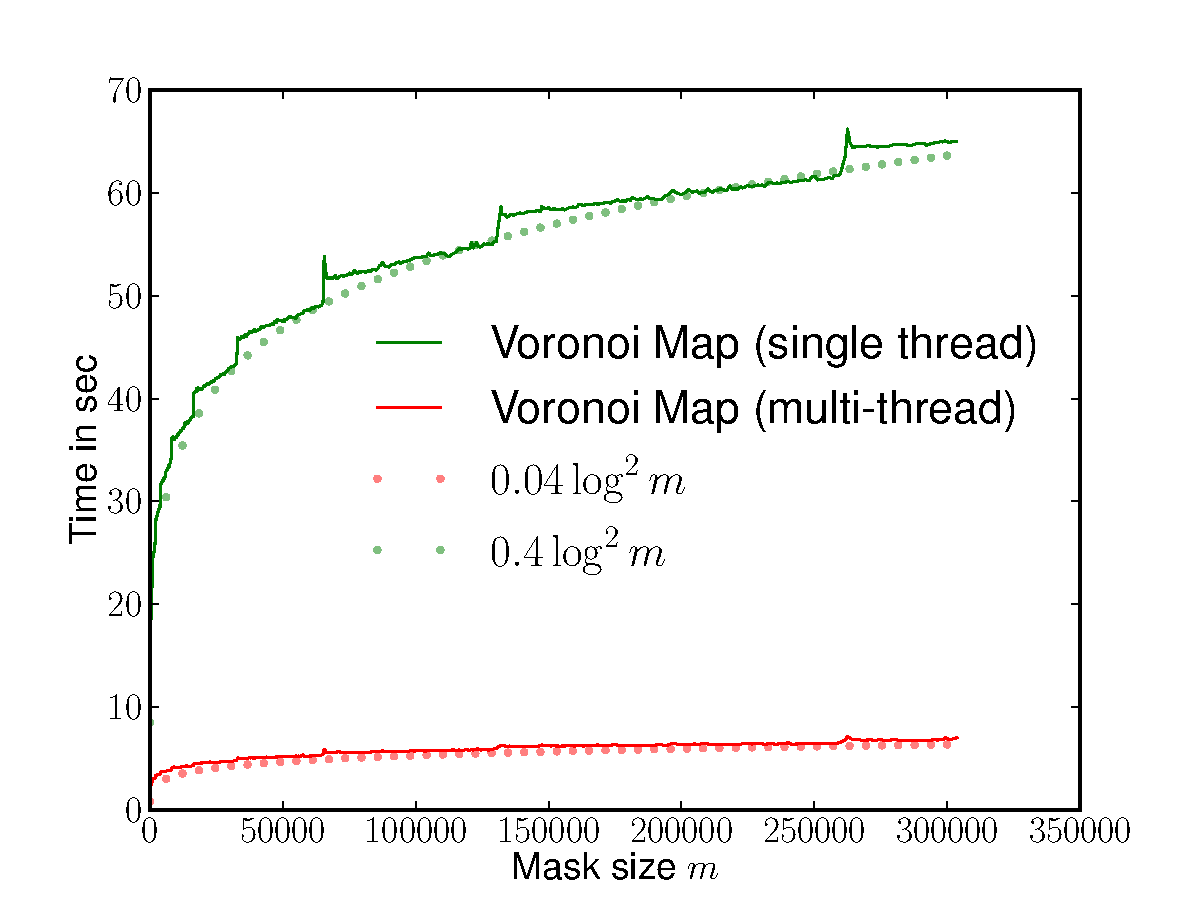
\includegraphics[width=\textwidth]{data/result}
  \caption{Experimental evaluation of subquadratic chamfer norm
    Voronoi map computation.}
  \label{fig:graph}
\end{figure}
In Fig.\ref{fig:graph}, we have considered a 2D domain $2048^2$ with
$2048$ random sites (and chamfer norm with increasing size
$m$). First, we observe that fixing $N$, the $\log^2{m}$ term is
clearly visible in the computational cost of the Voronoi map (single
thread curve). Bumps in the single thread curve may be due to memory
cache issues. Please note that if we consider classical chamfer norm
DT from raster scan (and half-masks), the computational cost would
have been in $O(m\cdot N^2)$ and thus would have a linear behavior in
Fig.~\ref{fig:graph}.

Since we have a separable algorithm, we can trivially implement it in
a multi-thread environment. Hence, on a bi-processor and quad-core
(hyperthreading) Intel(R) Xeon(R) cpu (16 threads can run in
parallel), we observe a speed-up by a factor 10 (multi-thread) curve
in Fig.~\ref{fig:graph}).

Please note that on this $2048^2$ domain with 2048 sites, Euclidean
Voronoi Map ($L_2$) is obtained in  954.837 milliseconds on a single
core and 723.196 msec on 16 cores.



\section{Discussion}
\label{sec:discussion}

\bibliographystyle{splncs}
\bibliography{library,mybiblio,dtbib}
\end{document}
